\documentclass{beamer}
%Information to be included in the title page:
% \title{Sample title}
% \author{Anonymous}
% \institute{Overleaf}
\usepackage{xcolor}
\usepackage{booktabs}
\usepackage{graphicx}
\usepackage{subcaption}
\usepackage[]{hyperref}

\usetheme[]{default}
\begin{document}
\renewcommand{\d}{\: \mathrm{d} }
\newcommand{\e}{\mathrm{e}}


\title[] {Recitation Class 6}

\author[lzx]{Zexi Li}

\institute[email]{lzx12138@sjtu.edu.cn}

\date{2021.06.29}

\frame{\titlepage}

\AtBeginSection[]
{
    \begin{frame}
        \frametitle{Table of Contents}
        \tableofcontents[currentsection]
    \end{frame}
}

\begin{frame}
    \frametitle{Outline}
    \tableofcontents
\end{frame}

\section{Chapter 7-II The pn Junction}
    \begin{frame} \frametitle{Reverse Applied Bias}
        \begin{figure}[H]
            \centering
            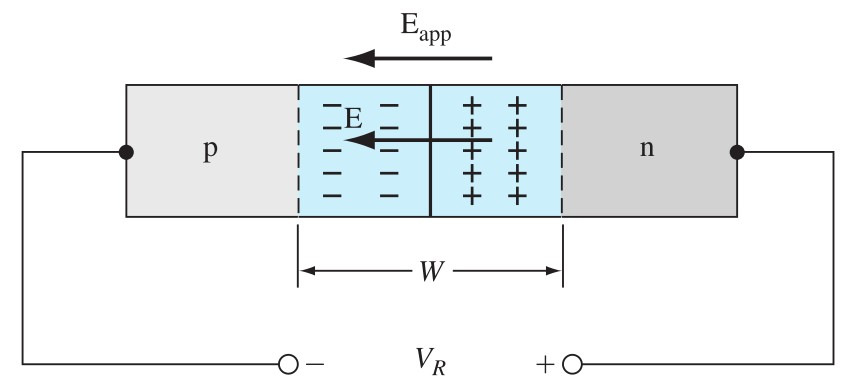
\includegraphics[width=0.5\linewidth]{Reversed-biase-graph.jpg}
            \label{fig:Reversed-biase-graph.jpg}
        \end{figure}
        \begin{figure}[H]
            \centering
            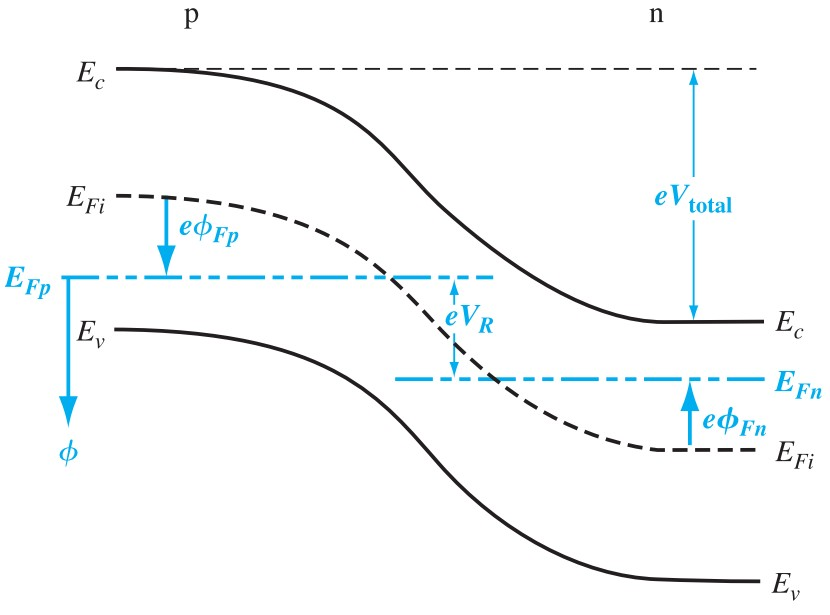
\includegraphics[width=0.5\linewidth]{Energy-band-diagram-reversed-biase.jpg}
            \caption{Energy-band diagram}
            \label{fig:Energy-band-diagram-reversed-biase.jpg}
        \end{figure}
    \end{frame}


    \begin{frame} \frametitle{From RC 5}
        \fbox{
        \begin{minipage}{0.95\linewidth}
            \begin{equation*}
                N_a x_p = N_d x_n
            \end{equation*}
            \begin{equation*}
                \begin{aligned}
                    x_n &= \sqrt{\frac{2 \varepsilon_s \left( V_{bi} + V_R \right)}{e} \left[ \frac{N_a}{N_d}  \right]\left[ \frac{1}{N_a + N_d}  \right]} \\
                    x_p &= \sqrt{\frac{2 \varepsilon_s \left( V_{bi} + V_R \right)}{e} \left[ \frac{N_d}{N_a}  \right]\left[ \frac{1}{N_a + N_d}  \right]}
                \end{aligned}
            \end{equation*}
            \par $\varepsilon_s = \varepsilon_r \varepsilon_0$, where $\varepsilon_0 = 8.85 \times 10^{-14} F \cdot cm^{-1}$.
            \par $\varepsilon_r = 11.7$ for $Si$.

            \begin{equation*}
                W = x_n + x_p = \sqrt{\frac{2 \varepsilon_s \left( V_{bi} + V_R \right)}{e}  \left[ \frac{N_a + N_d}{N_a N_d}  \right]}
            \end{equation*}
        \end{minipage}
        }
    \end{frame}
    \begin{frame} \frametitle{From RC 5}
        \fbox{
        \begin{minipage}{0.95\linewidth}
            \begin{equation*}
                E = \left\{
                    \begin{aligned}
                        - \frac{eN_a}{\varepsilon_s} (x + x_p),\quad & - x_p \le x \le 0 \\
                        \frac{eN_d}{\varepsilon_s} (x_n - x),\quad & 0 \le x \le x_n  
                    \end{aligned}
                \right.
            \end{equation*}
            \begin{equation*}
                \begin{aligned}
                    |E_{max}| &= - \frac{eN_d x_n}{\varepsilon_s} = - \frac{e N_a x_p}{\varepsilon_s} \\ 
                    &= - \frac{2 (V_{bi} + V_R)}{W} 
                \end{aligned}
            \end{equation*}
            \begin{equation*}
                \phi(x) = - \int E(x) \d x
            \end{equation*}
        \end{minipage}
        }
    \end{frame}
    \begin{frame}{From RC 5}
        \begin{minipage}{\linewidth}
            \begin{minipage}[b]{0.49\linewidth}
                \begin{figure}[H]
                    \centering
                    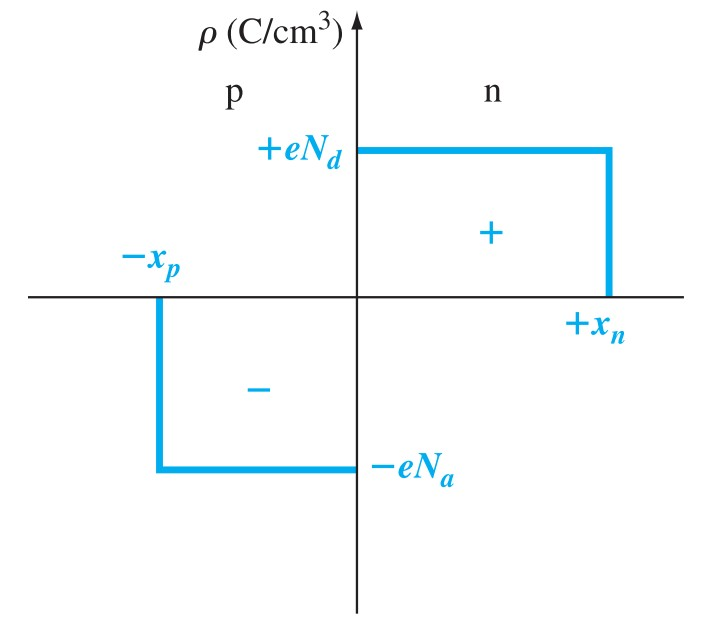
\includegraphics[width=0.95\linewidth]{Space-charge-density.jpg}
                    \caption{space charge density}
                    \label{fig:Space-charge-density.jpg}
                \end{figure}
                \begin{equation*}
                    N_a x_p = N_d x_n
                \end{equation*}
            \end{minipage}
            \begin{minipage}[b]{0.49\linewidth}
                \begin{figure}[H]
                    \centering
                    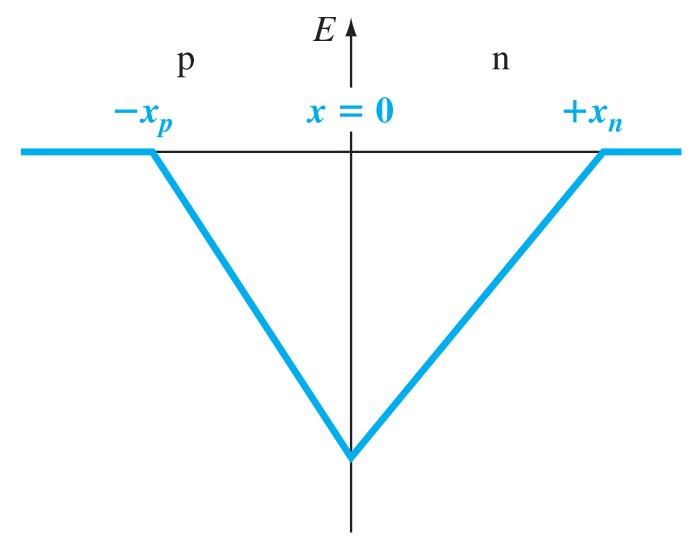
\includegraphics[width=0.95\linewidth]{pn-junction-electric-field.jpg}
                    \caption{electric field}
                    \label{fig:pn-junction-electric-field.jpg}
                \end{figure}
                \begin{equation*}
                    |k| = \frac{e N_{a/d}}{\varepsilon_s} 
                \end{equation*}
            \end{minipage}
        \end{minipage}
    \end{frame}

    \begin{frame} \frametitle{Junction Capacitance}
        \begin{figure}[H]
            \centering
            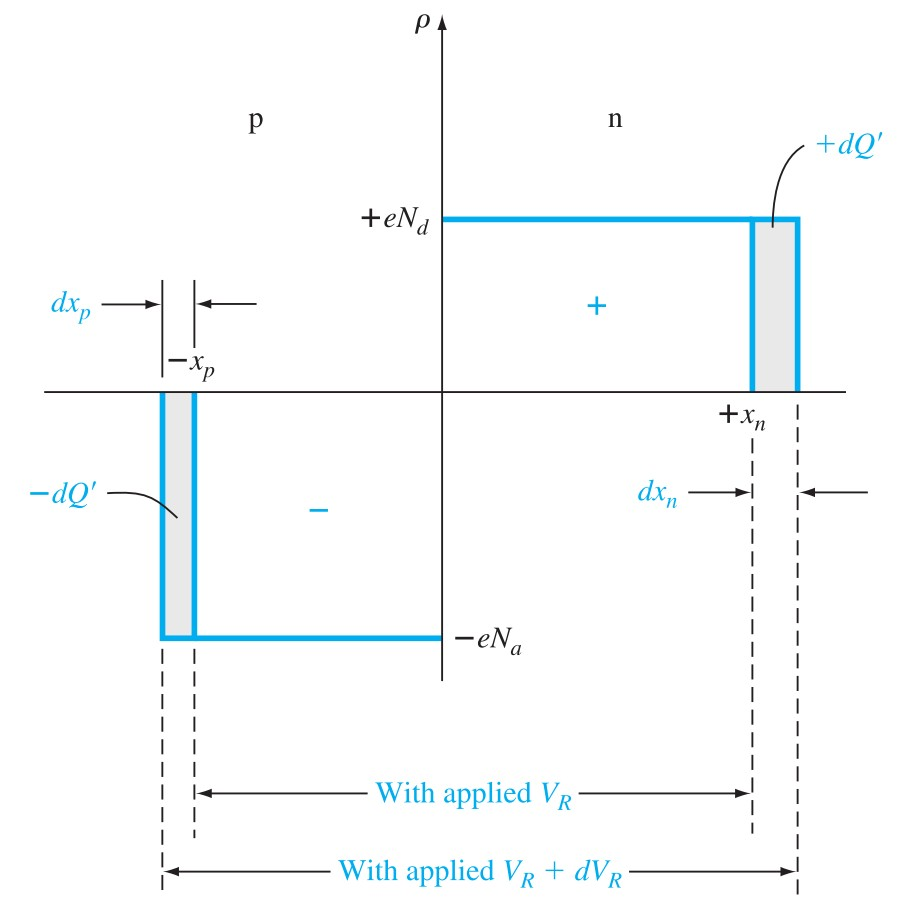
\includegraphics[width=0.6\linewidth]{Junction-capacitance.jpg}
            \caption{Differential change in the space charge width with a differential change in reverse-biased voltage for a uniformly doped pn junction}
            \label{fig:Junction-capacitance.jpg}
        \end{figure}
    \end{frame}

    \begin{frame} \frametitle{Junction Capacitance}
        \begin{equation*}
            \begin{aligned}
                C^\prime &= \frac{\d Q^\prime}{d V_R} \\
                d Q^\prime &= e N_d \d x_n = e N_a \d x_p
            \end{aligned}
        \end{equation*}
        \textcolor{orange}{$\d Q^\prime$ has units of $C/cm^2$, and $C^\prime$ has units of $F/cm^2$}.
        \begin{equation*}
            \boxed{C^\prime = \sqrt{\frac{e \varepsilon_s N_a N_d}{2 (V_{bi} + V_R) (N_a + N_d)} } = \frac{\varepsilon_s}{W} }
        \end{equation*}
    \end{frame}

    \begin{frame} \frametitle{One-sided Junction}
        \begin{minipage}{\linewidth}
            \begin{minipage}{0.5\linewidth}
                \par p$^+$n junction, $N_a \gg N_d$.
                \begin{equation*}
                    \begin{aligned}
                        & x_{p} \ll x_n \\
                        & W \approx x_n \\
                        & C^\prime \approx \sqrt{\frac{e \varepsilon_s N_d}{2 (V_{bi} + V_R)} } 
                    \end{aligned}
                \end{equation*}
            \end{minipage}
            \begin{minipage}{0.4\linewidth}
                \begin{figure}[H]
                    \centering
                    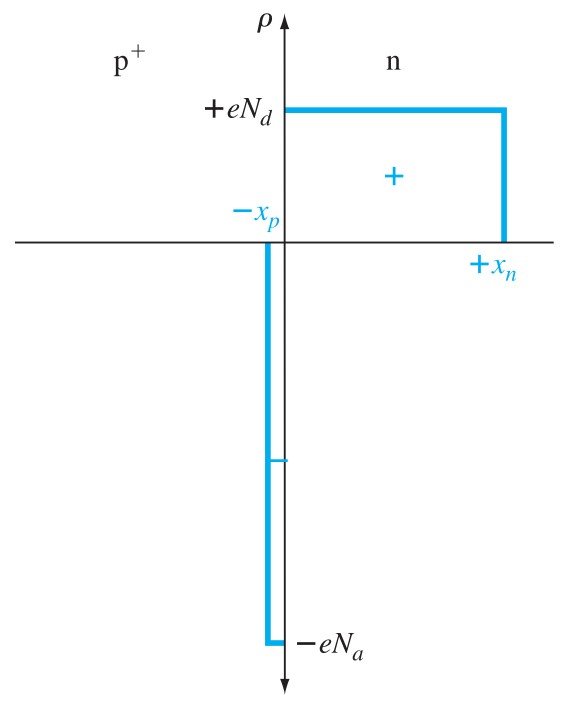
\includegraphics[width=\linewidth]{One-sided-junction.jpg}
                    \caption{Space charge density of a one-sided p$^+$n junction.}
                    \label{fig:One-sided-junction.jpg}
                \end{figure}
            \end{minipage}
        \end{minipage}
    \end{frame}
    \begin{frame} \frametitle{One-sided Junciton}
        \begin{minipage}{\linewidth}
            \begin{minipage}{0.5\linewidth}
                \begin{equation*}
                    \begin{aligned}
                        & C^\prime \approx \sqrt{\frac{e \varepsilon_s N_d}{2 (V_{bi} + V_R)} } \\
                        \Rightarrow & \boxed{\left( \frac{1}{C^\prime}  \right)^2 = \frac{2(V_{bi} + V_R)}{e \varepsilon_s N_d} }
                    \end{aligned}
                \end{equation*}
                Experimentally determine $V_{bi}$ and $N_d$.
            \end{minipage}
            \hspace{2em}
            \begin{minipage}{0.4\linewidth}
                \begin{figure}[H]
                    \centering
                    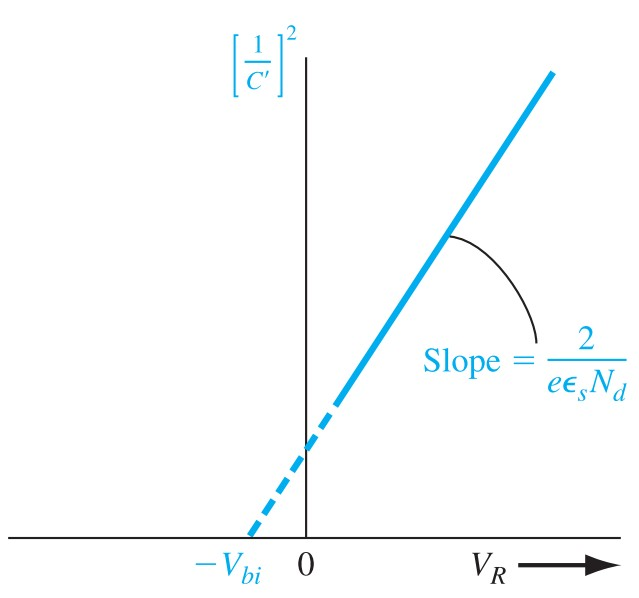
\includegraphics[width=\linewidth]{C-versus-VR.jpg}
                    \caption{$(1/C^\prime)^2$ versus $V_R$ of a \textcolor{orange}{uniformly} doped pn junction}
                    \label{fig:C-versus-VR.jpg}
                \end{figure}
            \end{minipage}
        \end{minipage}
    \end{frame}

\section{Chapter 8-I The pn Junction Diode}
    \begin{frame} \frametitle{Notations}
        \begin{figure}[H]
            \centering
            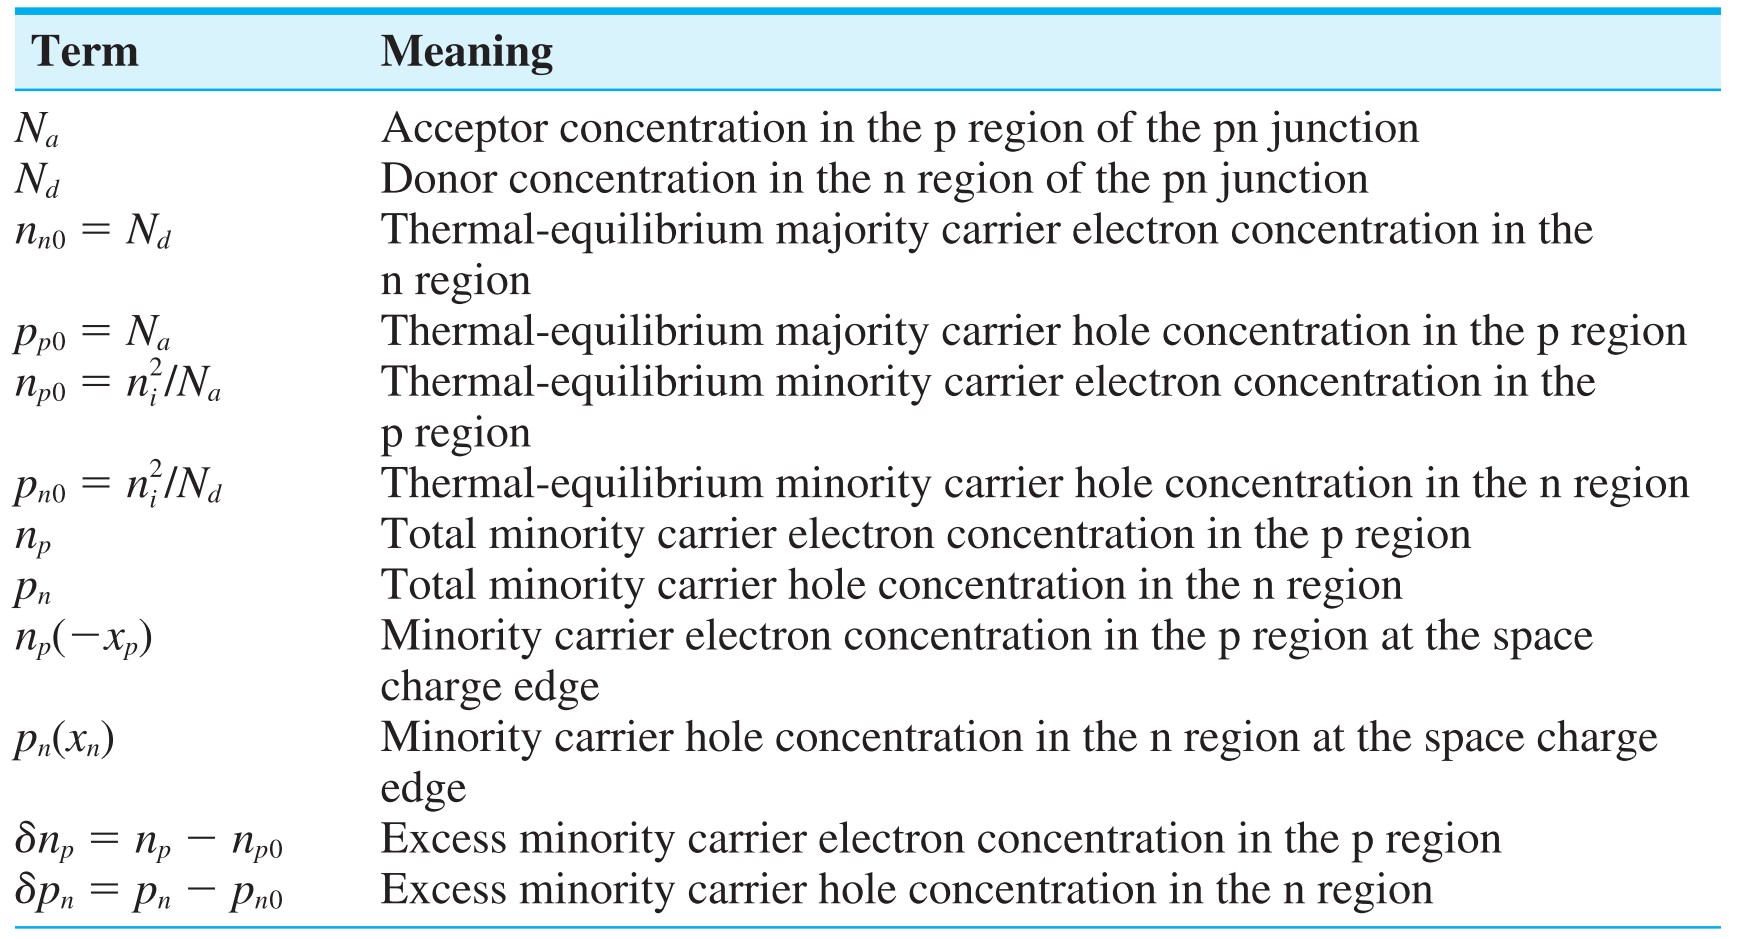
\includegraphics[width=0.9\linewidth]{Chapter-8-notations.jpg}
            \label{fig:Chapter-8-notations.jpg}
        \end{figure}
    \end{frame}

    \begin{frame} \frametitle{Ideal Current–Voltage Relationship}
        \begin{enumerate}[1.]
            \item The abrupt depletion layer approximation applies. The space charge regions have abrupt boundaries, and the semiconductor is neutral outside of the depletion region.
            \item The Maxwell–Boltzmann approximation applies to carrier statistics. 
            \item The concepts of low injection and complete ionization apply.
            \item \begin{enumerate}[a)]
                \item The total current is a constant throughout the entire pn structure. 
                \item The individual electron and hole currents are continuous functions through the pn structure.
                \item The individual electron and hole currents are constant throughout the depletion region.
            \end{enumerate}
        \end{enumerate}
    \end{frame}

    \begin{frame} \frametitle{Concentration Relation on Two Sides}
        \begin{equation*}
            \begin{aligned}
                V_{bi} &= V_t \ln \left( \frac{N_a N_d}{n_i^2}  \right)\\
                n_{n0} & \approx N_d \\
                n_{p0} & \approx \frac{n_i^2}{N_a}  \\
                \Longrightarrow \quad n_{p0} &= n_{n0} \exp\left( -\frac{e V_{bi} }{kT}  \right)
            \end{aligned}
        \end{equation*}
        \par Relates the minority carrier electron concentration on the p side of the junction to the majority carrier electron concentration on the n side of the junction in thermal equilibrium.
    \end{frame}

    \begin{frame} \frametitle{Forward Biased}
        \begin{figure}[H]
            \centering
            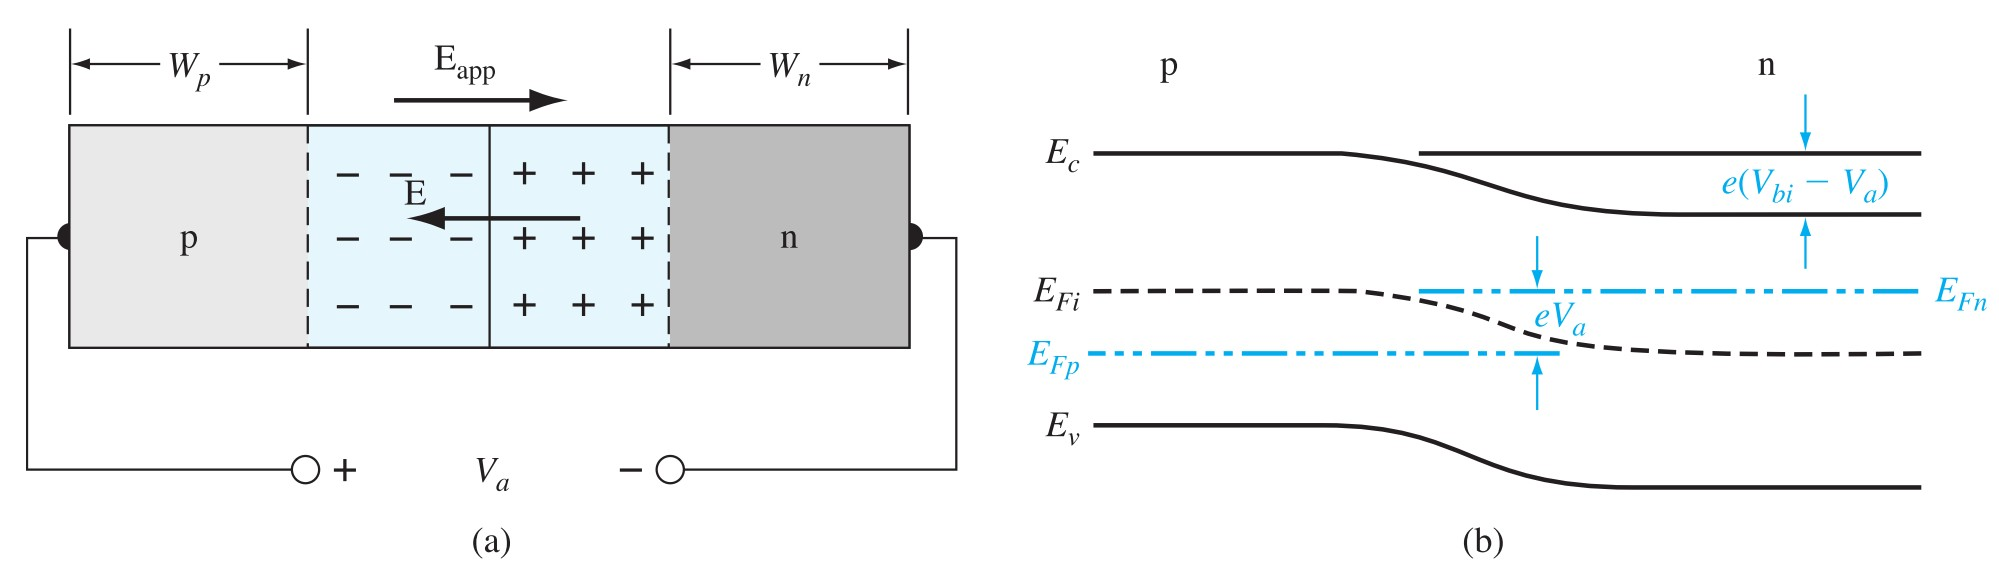
\includegraphics[width=0.9\linewidth]{Forward-biased-equation.jpg}
            \label{fig:Forward-biased-equation.jpg}
        \end{figure}
        \begin{equation*}
            \begin{aligned}
                n_p &= n_{n0} \exp\left( -\frac{e (V_{bi} - V_a)}{kT}  \right) \\
                &= n_{p0} \exp\left( \frac{eV_a}{kT}  \right)
            \end{aligned}
        \end{equation*}
    \end{frame}
    \begin{frame} \frametitle{Forward Biased}
        \begin{figure}[H]
            \centering
            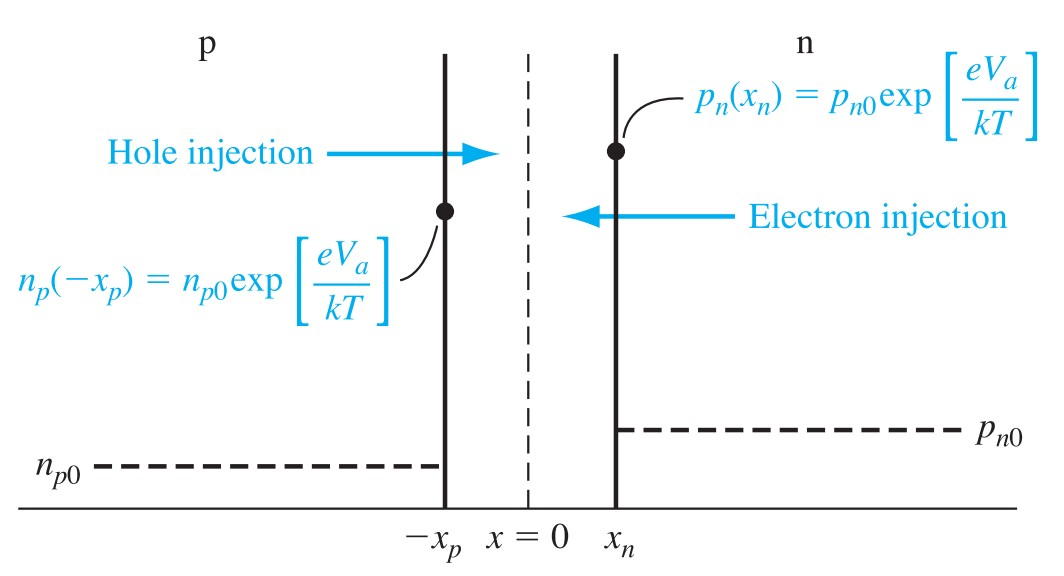
\includegraphics[width=0.8\linewidth]{Forward-biased-edge-concentration.jpg}
            \label{fig:Forward-biased-edge-concentration.jpg}
        \end{figure}
    \end{frame}

    \begin{frame} \frametitle{Minority Carrier Distribution}
        \begin{equation*}
            D_p \frac{\d^2 (\delta p_n)}{\d x^2} - \mu_p \left( E \frac{\d (\delta p_n)}{\d x} + p \frac{\d E}{\d x}  \right) + g^\prime- \frac{\delta p_n}{\tau_{pt}} = 0
        \end{equation*}
        \par Assumption: the electric field is zero in both the neutral p and n regions.
        \par In n region for $x > x_n$, we have $g^\prime = 0$.
        \par The equation becomes
        \begin{equation*}
            \frac{\d ^2 (\delta p_n)}{\d x^2} - \frac{\delta p_n}{L^2_p} = 0, \quad (x > x_n), \quad L_n^2 = D_n \tau_{n0} 
        \end{equation*}
        \par Solve it with boundary conditions
        \begin{equation*}
            \begin{aligned}
                & p_n(x_n) = p_{n0} \exp \left( \frac{eV_a}{kT}  \right)  \\
                & p_n (x \to +\infty) = p_{n0} 
            \end{aligned}
        \end{equation*}
    \end{frame}
    \begin{frame} \frametitle{Minority Carrier Distribution - Continue}
        The solution is
        \begin{equation*}
            \resizebox*{\textwidth}{!}{
                \boxed{\delta p_n(x) = p_n(x) - p_{n0} = p_{n0} \left[ \exp\left( \dfrac{eV_a}{kT} \right) - 1\right] \exp\left( \dfrac{x_n - x}{L_p}  \right), \quad x \ge x_n}
            }
        \end{equation*}
        Similarly,
        \begin{equation*}
            \resizebox*{\textwidth}{!}{
                \boxed{\delta n_p(x) = n_p(x) - n_{p0} = n_{p0} \left[ \exp\left( \dfrac{eV_a}{kT}  \right) - 1 \right] \exp \left( \dfrac{x_p + x}{L_n}  \right), \quad x \le - x_p}
            }
        \end{equation*}
        \begin{figure}[H]
            \centering
            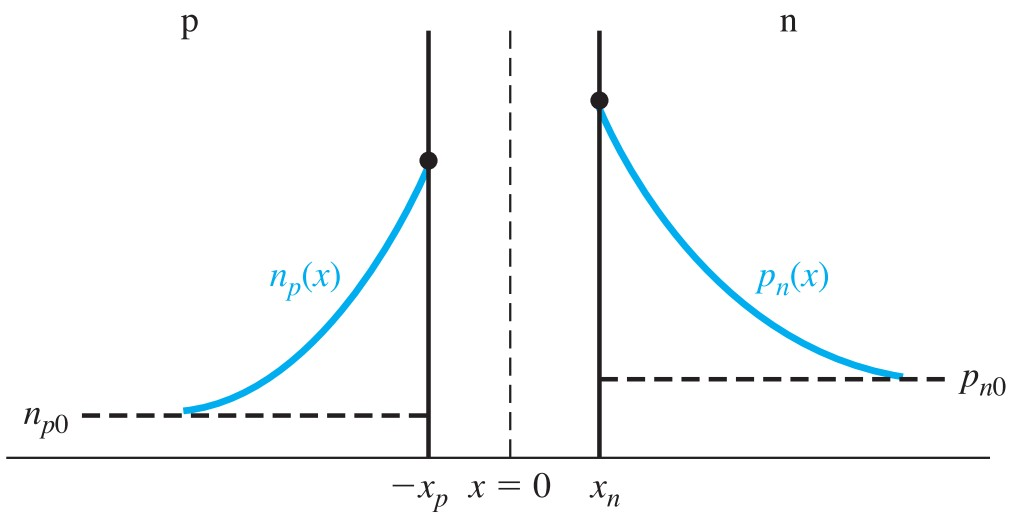
\includegraphics[width=0.6\linewidth]{Forward-biased-solution.jpg}
            \label{fig:Forward-biased-solution.jpg}
        \end{figure}
    \end{frame}

    \begin{frame} \frametitle{Quasi-Fermi Level}
        \begin{figure}[H]
            \centering
            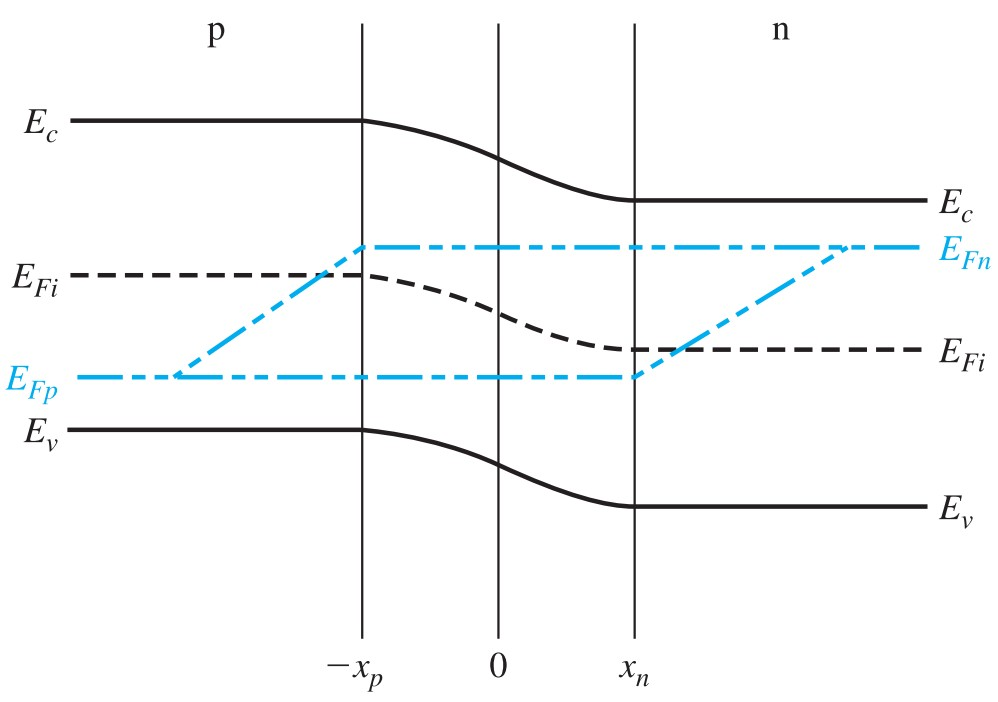
\includegraphics[width=0.5\linewidth]{Quasi-fermi-level.jpg}
            \caption{Quasi-Fermi levels through a forward-biased pn junction.}
            \label{fig:Quasi-fermi-level-1.jpg}
        \end{figure}
        % \vspace{-2em}
        \par In Chapter 6 there are equations
        \begin{equation*}
            p = p_0 + \delta p = n_i \exp\left( \frac{E_{Fi} - E_{Fp} }{kT}  \right)
        \end{equation*}
        \par Therefore the quasi-Fermi levels are linear functions of distance in the neutral p and n regions as shown in the Figure.
    \end{frame}
    \begin{frame} \frametitle{Quasi-Fermi Level - Continue}
        \begin{figure}[H]
            \centering
            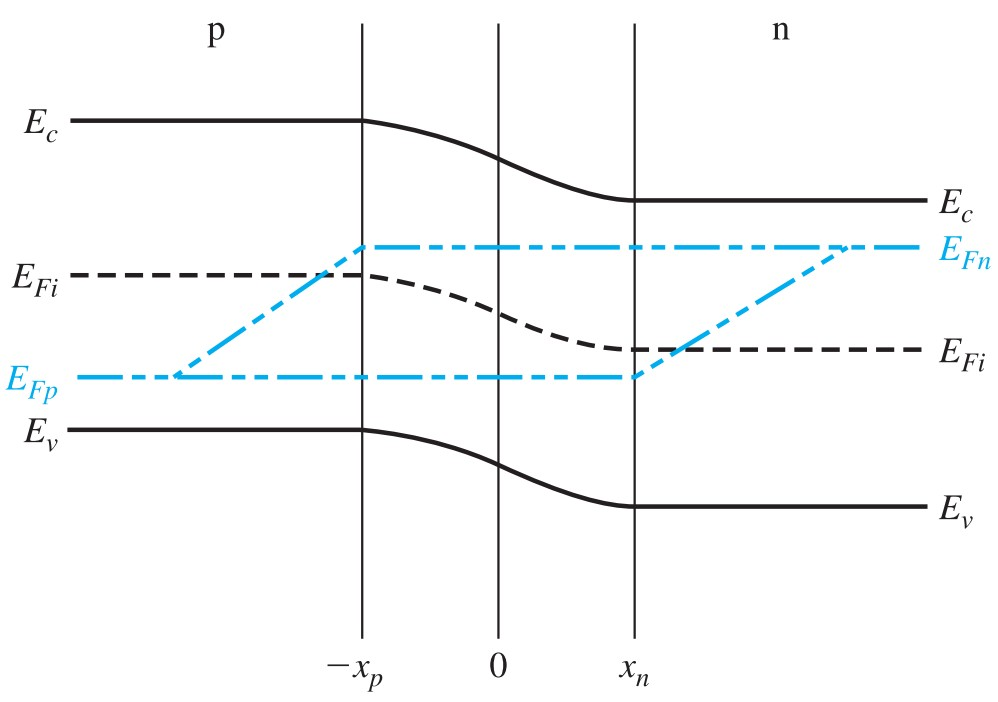
\includegraphics[width=0.5\linewidth]{Quasi-fermi-level.jpg}
            \caption{Quasi-Fermi levels through a forward-biased pn junction.}
            \label{fig:Quasi-fermi-level-2.jpg}
        \end{figure}
        \par Also, 
        \begin{equation*}
            np = n_i^2 \exp \left( \frac{E_{Fn} - E_{Fp} }{kT}  \right)
        \end{equation*}
    \end{frame}

    \begin{frame} \frametitle{Ideal pn Junction Current}
        \par Assumption 4(a): The total current is a constant throughout the entire pn structure.
        \begin{figure}[H]
            \centering
            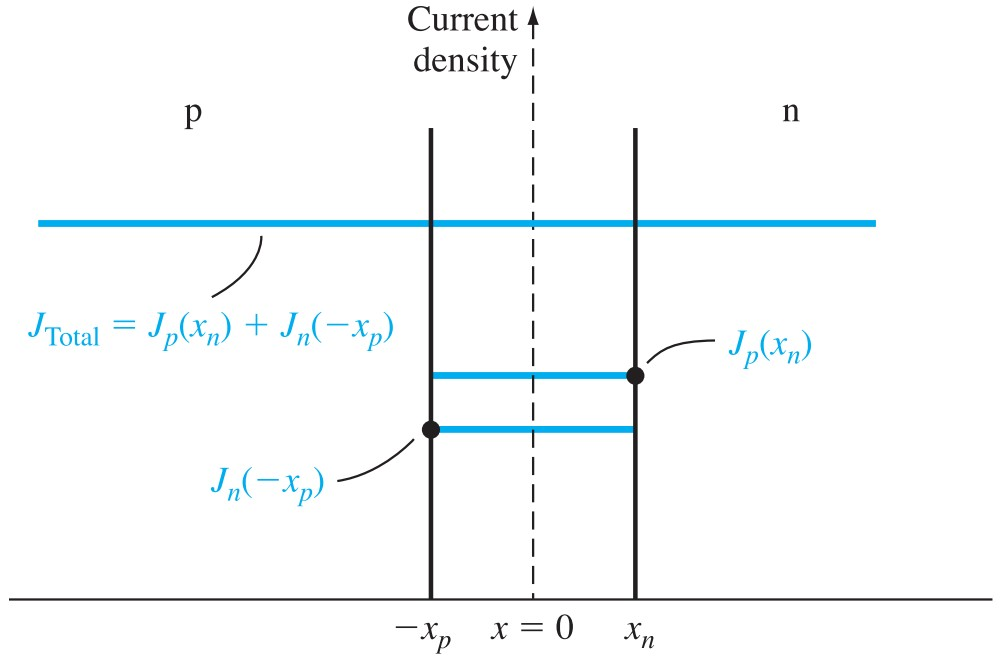
\includegraphics[width=0.6\linewidth]{Current-density.jpg}
            \label{fig:Current-density.jpg}
        \end{figure}
        \begin{equation*}
            J_p(x_n) = - e D_p \left. \frac{\d \left( \delta p_n(x) \right)}{\d x} \right|_{x = x_n}
        \end{equation*}
    \end{frame}
    \begin{frame} \frametitle{Ideal pn Junction Current - Continue}
        \begin{equation*}
            \begin{aligned}
                J_{p} (x_n) &= \frac{e D_p p_{n0}}{L_p} \left[ \exp\left( \frac{eV_a}{kT}  \right) - 1 \right] \\
                J_{n} (-x_p) &= \frac{eD_n n_{p0} }{L_n} \left[ \exp\left( \frac{eV_a}{kT}  \right) - 1 \right]
            \end{aligned}
        \end{equation*}
        \par Then the total current density
        \begin{equation*}
            \boxed{
                \begin{aligned}
                    J &= J_s \left[ \exp\left( \frac{eV_a}{kT}  \right) - 1 \right] \\
                    & \qquad  \text{where } J_s = \left[ \frac{eD_p p_{n0} }{L_p} + \frac{eD_n n_{p0} }{L_n}  \right]
                \end{aligned}
            }
        \end{equation*}
    \end{frame}

    \begin{frame} \frametitle{Ideal pn Junction Current - Continue}
        \begin{figure}[H]
            \centering
            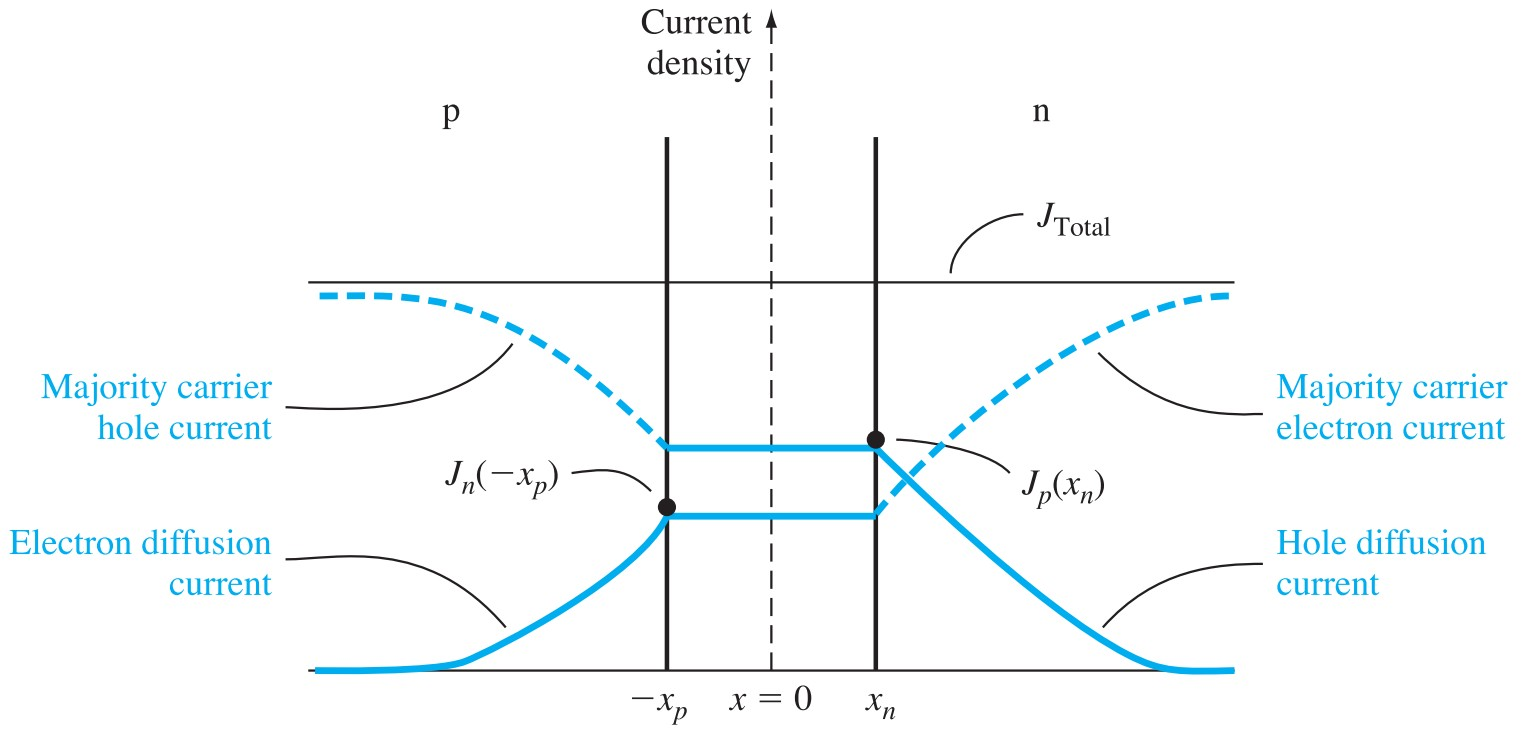
\includegraphics[width=0.9\linewidth]{Ideal-current-components.jpg}
            \caption{Idea electron and hole current components through a pn junction under forward bias.}
            \label{fig:Ideal-current-components.jpg}
        \end{figure}
    \end{frame}

    \begin{frame} \frametitle{Example}
        \par Consider the following parameters in a silicon pn junction at $T = 300K$:
        \begin{equation*}
            \begin{aligned}
                N_a &= N_d = 10^{16} cm^{-3} & n_i &= 1.5 \times 10^{10}  cm^{-3}  \\
                D_n &= 25 cm^{2} /s & \tau_{p0} &= \tau_{n0} = 5 \times 10^{-7} s \\
                D_p &= 10cm^2 / s &  \varepsilon_r &= 11.7 
            \end{aligned}
        \end{equation*}
        \begin{enumerate}[a)]
            \item Determine the ideal reverse-saturation current density.
            \item Calculate the electric field in a neutral region of a silicon diode to produce a given majority carrier drift current density.
        \end{enumerate}
        (Textbook Example 8.2 \& 8.4)
    \end{frame}
    
    \begin{frame} \frametitle{Solution}
        Solution:
        \begin{enumerate}[a)]
            \item \fbox{\textcolor{white}{$J_s = 4.6 \times 10^{-11} A/cm^2$}} 
            \item \fbox{\textcolor{white}{$E = 1.525 V/cm$}}
        \end{enumerate}
        \par Comment:
        \begin{enumerate}[a)]
            \item The ideal reverse-biased saturation current density is very small.
            \item We assumed, in the derivation of the current–voltage equation, that the electric field in the neutral p and n regions was zero. Although the electric field is not zero, this example shows that the magnitude is very small—thus the approximation of zero electric field is very good.
        \end{enumerate}
    \end{frame}

    \begin{frame} 
        \begin{center}
            \Large\textcolor{blue}{End}
        \end{center}
    \end{frame}
\end{document} 